\documentclass[11pt,dvipsnames,enabledeprecatedfontcommands]{scrartcl}
\usepackage{lmodern}
\usepackage{amssymb,amsmath}
\usepackage{ifxetex,ifluatex}
\usepackage{fixltx2e} % provides \textsubscript
\ifnum 0\ifxetex 1\fi\ifluatex 1\fi=0 % if pdftex
  \usepackage[T1]{fontenc}
  \usepackage[utf8]{inputenc}
\else % if luatex or xelatex
  \ifxetex
    \usepackage{mathspec}
  \else
    \usepackage{fontspec}
  \fi
  \defaultfontfeatures{Ligatures=TeX,Scale=MatchLowercase}
\fi
% use upquote if available, for straight quotes in verbatim environments
\IfFileExists{upquote.sty}{\usepackage{upquote}}{}
% use microtype if available
\IfFileExists{microtype.sty}{%
\usepackage[]{microtype}
\UseMicrotypeSet[protrusion]{basicmath} % disable protrusion for tt fonts
}{}
\PassOptionsToPackage{hyphens}{url} % url is loaded by hyperref
\usepackage[unicode=true]{hyperref}
\PassOptionsToPackage{usenames,dvipsnames}{color} % color is loaded by hyperref
\hypersetup{
            pdftitle={Rethinking legal probabilism},
            pdfauthor={Rafał Urbaniak},
            colorlinks=true,
            linkcolor=Maroon,
            citecolor=Blue,
            urlcolor=blue,
            breaklinks=true}
\urlstyle{same}  % don't use monospace font for urls
\usepackage{graphicx,grffile}
\makeatletter
\def\maxwidth{\ifdim\Gin@nat@width>\linewidth\linewidth\else\Gin@nat@width\fi}
\def\maxheight{\ifdim\Gin@nat@height>\textheight\textheight\else\Gin@nat@height\fi}
\makeatother
% Scale images if necessary, so that they will not overflow the page
% margins by default, and it is still possible to overwrite the defaults
% using explicit options in \includegraphics[width, height, ...]{}
\setkeys{Gin}{width=\maxwidth,height=\maxheight,keepaspectratio}
\IfFileExists{parskip.sty}{%
\usepackage{parskip}
}{% else
\setlength{\parindent}{0pt}
\setlength{\parskip}{6pt plus 2pt minus 1pt}
}
\setlength{\emergencystretch}{3em}  % prevent overfull lines
\providecommand{\tightlist}{%
  \setlength{\itemsep}{0pt}\setlength{\parskip}{0pt}}
\setcounter{secnumdepth}{5}
% Redefines (sub)paragraphs to behave more like sections
\ifx\paragraph\undefined\else
\let\oldparagraph\paragraph
\renewcommand{\paragraph}[1]{\oldparagraph{#1}\mbox{}}
\fi
\ifx\subparagraph\undefined\else
\let\oldsubparagraph\subparagraph
\renewcommand{\subparagraph}[1]{\oldsubparagraph{#1}\mbox{}}
\fi

% set default figure placement to htbp
\makeatletter
\def\fps@figure{htbp}
\makeatother

%\documentclass{article}

% %packages
 \usepackage{booktabs}

\usepackage{multirow}
\usepackage{multicol}

\usepackage{graphicx}
\usepackage{longtable}
\usepackage{ragged2e}
\usepackage{etex}
%\usepackage{yfonts}
\usepackage{marvosym}
\usepackage[notextcomp]{kpfonts}
\usepackage{nicefrac}
\newcommand*{\QED}{\hfill \footnotesize {\sc Q.e.d.}}
\usepackage{floatrow}



\usepackage[textsize=scriptsize, textwidth = 1.5cm]{todonotes}
%\linespread{1.5}


\setlength{\parindent}{10pt}
\setlength{\parskip}{1pt}


%language
\usepackage{times}
\usepackage{t1enc}
%\usepackage[utf8x]{inputenc}
%\usepackage[polish]{babel}
%\usepackage{polski}

\usepackage{mathptmx}
\usepackage[scaled=0.88]{helvet}


%AMS
\usepackage{amsfonts}
\usepackage{amssymb}
\usepackage{amsthm}
\usepackage{amsmath}
\usepackage{mathtools}

\usepackage{geometry}
 \geometry{a4paper,left=20mm,top=15mm,bottom = 20mm, right = 20mm}


%environments
\newtheorem{fact}{Fact}



%abbreviations
\newcommand{\ra}{\rangle}
\newcommand{\la}{\langle}
\newcommand{\n}{\neg}
\newcommand{\et}{\wedge}
\newcommand{\jt}{\rightarrow}
\newcommand{\ko}[1]{\forall  #1\,}
\newcommand{\ro}{\leftrightarrow}
\newcommand{\exi}[1]{\exists\, {_{#1}}}
\newcommand{\pr}[1]{\mathsf{P}(#1)}
\newcommand{\cost}{\mathsf{cost}}


\newcommand{\odds}{\mathsf{Odds}}
\newcommand{\ind}{\mathsf{Ind}}
\newcommand{\nf}[2]{\nicefrac{#1\,}{#2}}
\newcommand{\R}[1]{\texttt{#1}}
\newcommand{\prr}[1]{\mbox{$\mathtt{P}_{prior}(#1)$}}
\newcommand{\prp}[1]{\mbox{$\mathtt{P}_{posterior}(#1)$}}



\newtheorem{q}{\color{blue}Question}
\newtheorem{lemma}{Lemma}
\newtheorem{theorem}{Theorem}



%technical intermezzo
%---------------------

\newcommand{\intermezzoa}{
	\begin{minipage}[c]{13cm}
	\begin{center}\rule{10cm}{0.4pt}



	\tiny{\sc Optional Content Starts}
	
	\vspace{-1mm}
	
	\rule{10cm}{0.4pt}\end{center}
	\end{minipage}\nopagebreak 
	}


\newcommand{\intermezzob}{\nopagebreak 
	\begin{minipage}[c]{13cm}
	\begin{center}\rule{10cm}{0.4pt}

	\tiny{\sc Optional Content Ends}
	
	\vspace{-1mm}
	
	\rule{10cm}{0.4pt}\end{center}
	\end{minipage}
	}
%--------------------

\DeclareUnicodeCharacter{0301}{*************************************}




















\newtheorem*{reply*}{Reply}
\usepackage{enumitem}
\newcommand{\question}[1]{\begin{enumerate}[resume,leftmargin=0cm,labelsep=0cm,align=left]
\item #1
\end{enumerate}}

\usepackage{float}

% \setbeamertemplate{blocks}[rounded][shadow=true]
% \setbeamertemplate{itemize items}[ball]
% \AtBeginPart{}
% \AtBeginSection{}
% \AtBeginSubsection{}
% \AtBeginSubsubsection{}
% \setlength{\emergencystretch}{0em}
% \setlength{\parskip}{0pt}






\usepackage[authoryear]{natbib}

%\bibliographystyle{apalike}

\title{Rethinking legal probabilism}
\author{Rafał Urbaniak}
\date{}

\begin{document}
\maketitle

\thispagestyle{empty}

\section{Scientific goal}\label{scientific-goal}

As many miscarriages of justice indicate, scientific evidence is easily
misinterpreted in court. This happens partially due to miscommunication
between the parties involved, partially due to the usual probabilistic
fallacies, but also because incorporating scientific evidence in the
context of a whole case can be really hard. Probabilistic tools for
piecemeal evaluation of scientific evidence and spotting probabilistic
fallacies in legal contexts are quite well developed. Yet, the
construction of a more general probabilistic model of incorporating such
evidence in a wider context of a whole case, useful for theorizing about
evidence evaluation and legal decision standards, remains a challenge.
Legal probabilism (LP), for our purpose, is the view that this challenge
can and should be met. This project intends to contribute to further
development of this enterprise in a philosophically motivated manner.

The assessment of evidence in the court of law can be viewed from at
least three perspectives: as an interplay of arguments, as an assessment
of probabilities involved, or as an interaction of competing narrations.
Each perspective presents an account of legal reasoning (Di Bello \&
Verheij, 2018; van Eemeren \& Verheij, 2017). Individually, each of
these strains has been investigated. The probabilistic approach, while
being fairly mature, is still underdeveloped in light of various lines
of criticism developed by the representatives of the other strains.

The \textbf{goal of this project} is to
\textbf{develop of a probabilistic and yet narration-based  modelling method of the  interaction of various items of evidence and hypotheses and the resulting decisions in the court of law}.
This will be achieved by accomodating important
\textbf{insights provided by the critics of legal probabilism}. A
crucial point of criticism is that the fact-finding process should be
conceptualized as \textbf{a competition of narrations}. Another point
comes from the argumentation theory framework: an adequate model should
capture the structure of the arguments involved and the interplay
between them, and it is not clear how this is to be achieved within the
probabilistic approach. The key idea is to represent
\textbf{narrations  as bayesian networks. Then, the argumentative structure becomes clear,  and various features requested by the critics can be explicated in terms of corresponding properties of,  operations on, and relations between bayesian networks}.
Thus, the goals are three-fold:

\begin{enumerate}
\def\labelenumi{\arabic{enumi}.}
\item
  Philosophical and conceptual improvement of legal probabilism by
  including a more holistic perspective and adversarial character of
  evidence assessment, which are typically absent from probabilistic
  approaches.
\item
  Formulation of a formal and computational probabilistic framework that
  incorporates features resulting from achieving goal 1. This will be
  done using Bayesian networks, hierarchical Bayesian models and
  imprecise probabilities. (\textbf{\textsf{R}} code capturing the
  technical features developed will be made openly available.)
\item
  Addressing the question of how evidence of different types can be
  aggregated and how adjudication should proceed in the presence of
  multiple competing narrations of what happened. The research in 1. and
  2. will help to address this very practical and pressing question.
\end{enumerate}

The output will be a
\textbf{unifying extended probabilistic model embracing key aspects of the narrative and argumentative approaches, , with  implementation in the programming language \textbf{\textsf{R}}.}\\
What the project will uniquely bring to the table is joining the
familiarity with epistemological debates, familiarity with the details
of evidence assessment in legal cases and technical skill to
programmatically implement, simulate and test various theoretical moves.

\pagebreak 

\section{Significance}\label{significance}

\subsection{State of the art}\label{state-of-the-art}

\subsubsection{Legal probabilism}\label{legal-probabilism}

From among the three perspectives already mentioned, the probablistic
approach will be my point of departure, for the following key reasons:

\begin{itemize}
\item
  The project is to be informed by and reflect on the actual practice of
  legal evidence evaluation, and much of scientific evidence in such
  contexts has probabilistic form.
\item
  Probabilistic tools are fairly well-developed both for applications
  and within formal epistemology, reaching a state of fruition which
  should inspire deeper reflection.
\item
  Statistical computing tools for such methods are available, which
  allows for programming development and preliminary computational and
  data-driven evaluation of the ideas to be defended.
\end{itemize}

Accordingly, the view in focus of this research is legal probabilism
(LP)---an ongoing research program that comprises a variety of claims
about evidence assessment and decision-making at trial. At its simplest,
it comprises two core tenets: first, that the evidence presented at
trial can be assessed, weighed and combined by means of probability
theory; and second, that legal decision rules, such as proof beyond a
reasonable doubt in criminal cases, can be explicated in probabilistic
terms.

The early theorists of probability in the 17th and 18th century were as
much interested in games of chance as they were interested in the
uncertainty of trial decisions (Bernoulli, 1713; Daston, 1988; Franklin,
2001; Hacking, 1975). Bernoulli's prescient insights attained greater
popularity in the 20th century amidst the law and economics movement
(Becker, 1968; Calabresi, 1961; Posner, 1973). Finkelstein \& Fairley
(1970) gave one of the first systematic analyses of how probability
theory, and Bayes' theorem in particular, can help to weigh evidence at
trial. Lempert (1977) was one of the first to propose to use likelihood
ratios for assessing the relevance of evidence. Such contributions
fueled what has been called the New Evidence Scholarship, a rigorous way
of studying the process of legal proof at trial (Lempert, 1986).

\subsubsection{Challenges to New Evidence
Scholarship}\label{challenges-to-new-evidence-scholarship}

Tribe (1971) attacked what he called `trial by mathematics', by listing
well-known cases of misuse or probabilities in legal contexts and
practical difficulties in assessing the probability of someone's
criminal or civil liability, and pointing out the dehumanization of
trial decisions that legal probabilism seems to propose. After Tribe,
many argued that probabilistic models are either inadequate or unhelpful
(Allen, 1986; Brilmayer, 1986; Cohen, 1986; Dant, 1988; Underwood,
1977). This negative trend has been somewhat mitigated by the discovery
of DNA fingerprinting in the eighties and progress in forensic science
in general, with the increasing role of quantitative evidence in the
court of law (Kaye, 1986, 2010; Koehler, 1996; National Research
Council, 1992; Robertson \& Vignaux, 1995).

Skepticism about wider mathematical and quantitative models of legal
evidence is still widespread among prominent legal scholars and
practitioners (see, for example, Allen \& Pardo, 2007). This is
partially in light of conceptual difficulties extensively discussed in
the literature, which arise when one wants to formulate a probabilistic
decision criterion for the court of law. Imagine you are a trier of fact
in a legal proceeding in which the defendant's guilt is identified as
equivalent to a certain factual statement \(G\) and that somehow you
succeeded in properly evaluating \(\pr{G\vert E}\)----the probability of
\(G\) given the total evidence presented to you, \(E\). One question
that arises in such a situation is: when should you decide against the
defendant? When is the evidence good enough? What we are after here is a
condition \(\Psi\), formulated in (primarily) probabilistic (and perhaps
decision-theoretic) terms, such that the trier of fact, at least
ideally, should accept any relevant claim \(A\) (including \(G\)) just
in case \(\Psi(A, E)\). One straightforward attempt might be to say:
convict if \(\pr{G\vert E}\) is above a certain threshold, otherwise
acquit (Dekay, 1996; Kaye, 1979; see, for example Laplace, 1814; Laudan,
2006).

This move, however, seems to be blocked by the so-called paradoxes of
legal proof or puzzles of naked statistical evidence. Nesson (1979),
Cohen (1981), and Thomson (1986) formulated scenarios in which, even if
the probability of guilt or civil liability, based on the available
evidence, is particularly high, a verdict against the defendant seems
unwarranted. A variant of such a scenario---the gatecrasher
paradox---goes as follows. Suppose our guilt threshold is high, say at
0.99. Consider the situation in which 1000 fans enter a football
stadium, and 991 of them avoid paying for their tickets. A random
spectator is tried for not paying. The probability that the spectator
under trial did not pay exceeds 0.99. Yet, intuitively, a spectator
cannot be considered liable on the sole basis of the number of people
who did and did not pay. While recently some doubt the relevance of
abstract philosophical examples for the actual practice (Hedden, 2019;
Ross, 2020), at least conceptual challenges remain.

Another conceptual problem is the so-called difficulty about
conjunction. It arises, because intuitively there should be no
difference between the trier's acceptance of \(A\) and \(B\) separately,
and her acceptance of their conjunction, \(A\wedge B\), that is, that
\(\Psi(A,E)\) and \(\Psi(B,E)\) just in case \(\Psi(A\wedge B, E)\). If
\(\Psi(H,E)\) is just the threshold criterion requiring that
\(\pr{H\vert E}\) be sufficiently high, \(\Psi\) in general fails to
satisfy this equivalence, as the probability of a conjunction generally
can be lower than the probability of any of the conjuncts.

Arguably, these problems underscore a theoretical difficulty with
probabilistic accounts of legal standards of proof. How to define them,
or whether they should be even defined in the first place, remains
contentious (Diamond, 1990; Horowitz \& Kirkpatrick, 1996; Laudan, 2006;
Newman, 1993; Walen, 2015). Judicial opinions offer different
paraphrases, sometimes conflicting, of what these standards mean. In the
last decade, philosophers have also joined the debate (Gardiner, 2018;
for critical surveys see Redmayne, 2008)

At least \emph{prima facie}, then, it seems that some conditions other
than high posterior probability of liability have to be satisfied for
the decision to penalize (or to find liable) to be justified.
Accordingly, various informal notions have been claimed to be essential
for a proper explication of judiciary decision standards (Haack, 2014;
Wells, 1992). For instance, evidence is claimed to be insufficient for
conviction if it is not \emph{sensitive} to the issue at hand: if it
remained the same even if the accused was innocent (Enoch \& Fisher,
2015). Or, to look at another approach, evidence is claimed to be
insufficient for conviction if it doesn't \emph{normically support} it:
if---given the same evidence---no explanation would be needed even if
the accused was innocent (Smith, 2017). A legal probabilist needs either
to show that these notions are unnecessary or inadequate for the purpose
at hand, or to indicate how they can be explicated in probabilistic
terms.

\subsubsection{The alternative
perspectives}\label{the-alternative-perspectives}

More recently, alternative frameworks for modeling evidential reasoning
and decision-making at trial have been proposed. They are based on
inference to the best explanation (Allen, 2010; Hastie, 2019; Ho, 2019;
Nance, 2019; Pardo \& Allen, 2008; Schwartz \& Sober, 2019), narratives
and stories (Allen, 1986, 2010; Allen \& Leiter, 2001; Clermont, 2015;
Pardo, 2018; Pennington \& Hastie, 1991a), and argumentation theory
(Bex, 2011; Gordon, Prakken, \& Walton, 2007; Walton, 2002). Those who
favor a conciliatory stance have combined legal probabilism with other
frameworks, offering preliminary sketches of hybrid theories (Urbaniak,
2018a; Verheij, 2014).

The main point of criticism is that legal proceedings are back-and-forth
between opposing parties in which cross-examination is of crucial
importance, reasoning goes not only evidence-to-hypothesis, but also
hypotheses-to-evidence (Allen \& Pardo, 2007; Wells, 1992) in a way that
seems analogous to inference to the best explanation (Dant, 1988), which
notoriously is claimed to not be susceptible to probabilistic analysis
(Lipton, 2004), and the process is an interaction of multiple arguments
that remain in fairly complicated relations. An informal philosophical
account inspired by such considerations---The
\textbf{No Plausible Alternative Story (NPAS)} theory (Allen, 2010)---is
that the courtroom is a confrontation of competing narrations (Ho, 2008;
Wagenaar, Van Koppen, \& Crombag, 1993) offered by the sides, and the
narrative to be selected should be the most plausible one. The view is
conceptually plausible (Di Bello, 2013), and finds support in
psychological evidence (Pennington \& Hastie, 1991b, 1992).

It would be a great advantage of LP if it could model phenomena captured
by the narrative approach. But how is the legal probabilist to make
sense of them? From her perspective, the key disadvantage of NPAS is
that it abandons the rich toolbox of probabilistic methods and takes the
key notion of plausibility to be a primitive notion which should be
understood only intuitively. It would be even better for LP if the
incorporation of such insights could lead to the resolution of the
already mentioned conceptual difficulties.

\subsubsection{Bayesian networks as a tool for legal
probabilism}\label{bayesian-networks-as-a-tool-for-legal-probabilism}

The idea that Bayesian networks can be used for probabilistic reasoning
in legal fact-finding started gaining traction in late eighties and
early nineties (Edwards, 1991), and it found its way to nowadays
standard textbooks on the topic (Fenton \& Neil, 2018a; Taroni,
Biedermann, Bozza, Garbolino, \& Aitken, 2014).\\
A Bayesian network comprises two components: first, a directed acyclic
graph of relations of dependence (represented by arrows) between
variables (represented by nodes); second, conditional probability
tables. Consider the graphical component first. The graph is acyclic
because the arrows connecting the nodes do not form loops. As an
illustration, let \(H\) be the claim that the suspect committed the
murder, \(BT\) the presence of a blood type B match with a crime scene
stain, and \(W\) the fact that an eyewitness observed the suspect near
the scene around the time of the crime. The graphical component of the
Bayesian network would look like this.

\noindent

\begin{tabular}{ll}
\begin{minipage}[c]{0.15\linewidth}
\begin{figure}[H]
\scalebox{0.9}{
\hspace{-10mm} \vspace{-5mm} 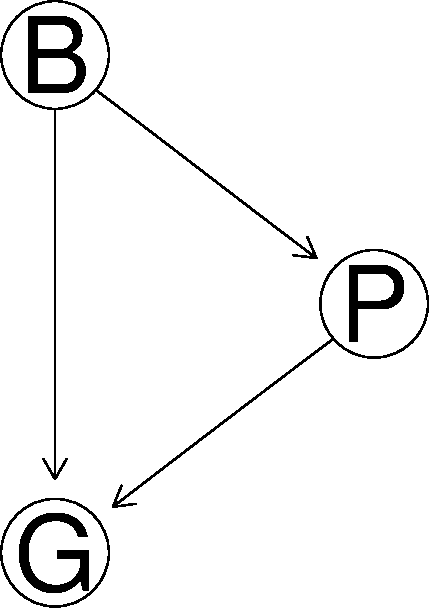
\includegraphics{BNfiles/unnamed-chunk-2-1}
}
\end{figure} \end{minipage}& \begin{minipage}[c]{0.795\linewidth}
The \emph{ancestors} of a node \(X\) are all those nodes from
which we can reach \(X\) by following the arrows going forwards. The
\textit{parents} of a node \(X\) are those for which we can do this in one step.
The \textit{descendants} of \(X\) are all which can be reached from \(X\) by
following the arrows going forward. The \textit{children} are those for
which we can do this in one step. In the example,
$H$ is the parent (and ancestor) of both $W$ and $BT$, which are its children (and descendants). There are no non-parent ancestors or non-children
descendants. 
\end{minipage}
\end{tabular}

\vspace{1mm}

The variables, which are represented by nodes and are connected by
arrows, stand in relation of probabilistic dependence. To describe these
relations, the graphical model is accompanied by conditional probability
tables. For instance, they can look as follows (the blood type frequency
estimate is realistic (Lucy, 2013), and so are the conditional
probabilities for the eyewitness identification, although for
complications about assessing eyewitness testimony see Wixted \& Wells
(2017) and Urbaniak, Kowalewska, Janda, \& Dziurosz-Serafinowicz
(2020)).

\noindent

\begin{tabular}{ll}
\begin{minipage}[c]{0.45\linewidth}
\begin{table}[H]
\centering
\begin{tabular}{lrr}
\toprule
  & H = murder & H=no.murder\\
\midrule
W = seen & .7 & .4\\
W = not.seen & .3 & .6\\
\bottomrule
\end{tabular}
\end{table}
\end{minipage}& \begin{minipage}[c]{0.45\linewidth}
\begin{table}[H]
\centering
\begin{tabular}{lrr}
\toprule
  & H = murder & H=no.murder\\
\midrule
BT = match & 1 & .063\\
BT = no.match & 0 & .937\\
\bottomrule
\end{tabular}
\end{table}
\end{minipage}
\end{tabular}

\vspace{2mm}

\noindent and a prior for the states of the root nodes (here, say,
\(\pr{H=murder} = .01\) and \(\pr{H= no.murder} = 0.99\)).

While the Bayesian network above---comprising a directed acyclic graph
along with probability tables---is simple, a correct intuitive
assessment of the probability of the hypothesis given the evidence is
already challenging. The reader is invited to try to estimate
intuitively the probability that the defendant committed the murder
(H=murder) given the following states of the evidence:

\begin{itemize} 
\item The suspect's blood type matches the crime stain but  information about the witness is unavailable.
\item The suspect's blood type matches the crime stain but the witness says they did not see the suspect near the crime scene.
\item The suspect's blood type matches the crime stain and the witness says they saw the suspect near the crime scene.
\end{itemize}

\vspace{1mm}

\begin{minipage}[c]{0.4\linewidth}
\begin{tabular}{lr}
\toprule
  & H=murder\\
\midrule
BT = match,W=? & .138\\
BT = match,W=not.seen & .074\\
BT = match, W=seen & .219\\
\bottomrule
\end{tabular}
\end{minipage}\begin{minipage}[c]{0.575\linewidth}
Already at this level of complexity, calculations by hand become cumbersome. In contrast,  software for Bayesian networks  will easily give the results visible on the left. Perhaps surprisingly, the posterior probability of $H$ is about .22 even when both pieces of evidence are incriminating (BT=match, W=seen).
\end{minipage}

\vspace{2mm}

In a similar vein, fairly simple graphical patterns (called
\emph{idioms}) often appear while modeling the relationships between
evidence and hypotheses. Complex graphical models can be constructed by
combining these basic patters in a modular way. Discussion of general
methods for Bayesian network constructions can be found in (Bovens \&
Hartmann, 2004; Friedman, 1974; Hepler, Dawid, \& Leucari, 2007; Neil,
Fenton, \& Nielson, 2000) and general idioms are discussed in (Fenton,
Neil, \& Lagnado, 2013).

Some attempts have been made to use Bayesian networks to weigh and
assess complex bodies of evidence consisting of multiple components. On
one hand, we have serious reconstructions of real complex cases. Kadane
\& Schum (2011) made one the first attempts to model an entire criminal
case, Sacco \& Vanzetti from 1920, using probabilistic graphs. Here is
another, more recent, example by Fenton \& Neil (2018b), who constructed
a Bayesian network for the famous Sally Clark case.

\noindent

\begin{tabular}{cc}
\begin{minipage}[c]{0.57\linewidth}
\begin{figure}[H]
\scalebox{1}{
\includegraphics{BNfiles/unnamed-chunk-11-1}  }
\end{figure}
\end{minipage} & \begin{minipage}[c]{0.37\linewidth}
The arrows depict relationships of influence between variables. Whether Sally Clark's sons, call them \(A\) and \(B\), died by SIDS or murder (\textsf{A.cause} and \textsf{B.cause}) influences whether signs of disease (\textsf{A.disease} and \textsf{B.disease}) and bruising (\textsf{A.bruising} and \textsf{B.bruising})  were present. 
Since son A died first, whether A was murdered or died by SIDS (\textsf{A.cause}) influences how son B died (\textsf{B.cause}). 
How the sons died 
determines how many sons were murdered (\textsf{No.murdered}), and how many sons were murdered decides whether Sally Clark is guilty (\textsf{guilty}). 
\end{minipage}
\end{tabular}

\vspace{2mm}

\noindent

\begin{tabular}{cc}
\begin{minipage}[c]{0.4\linewidth}
\begin{table}[H]
\centering
\begin{tabular}{@{}ll@{}}
\toprule
Evidence (cumulative) & $\pr{\textrm{Clark guilty}}$ 
\\ \midrule 
A bruising& .2887\\
A no signs of disease & .3093\\
B bruising & .6913\\
B no signs of disease  & .7019\\
 \bottomrule
\end{tabular}
\end{table}
\end{minipage} & \begin{minipage}[c]{0.54\linewidth}
In the  original calculation, the prior probability of \textrm{Guilty = Yes} should be .0789. After taking into account the incriminating evidence presented at trial, such as that there were signs of bruising but no signs of a preexisting disease affecting the children, the posterior probabilities are as in the table on the left.
\end{minipage}
\end{tabular}

\vspace{2mm}

The literature contains examples of more general methodological
reflection on the use of BNs for modeling whole cases. The main idea is
that once all the pieces of evidence and claims are represented as
nodes, one should use the \textit{scenario idiom} to model complex
hypotheses, consisting of a sequence of events organized in space and
time: a scenario (Vlek, Prakken, Renooij, \& Verheij, 2014). A
discussion of modelling crime scenarios by means of graphical devices
mixed with probabilities can be also found in the work of Shen, Keppens,
Aitken, Schafer, \& Lee (2007)\}, Bex (2011), Bex (2015) and Verheij
(2017). See also the survey by Di Bello \& Verheij (2018). Dawid \&
Mortera (2018) give a treatment of scenarios in terms of BNs.

A graphical model that uses the scenario idiom would consist of the
following components: first, nodes for the states and events in the
scenario, with each node linked to the supporting evidence; second, a
separate scenario node that has states and events as its children;
finally, a node corresponding to the ultimate hypothesis as a child of
the scenario node. Such a model could look like this:

\begin{center}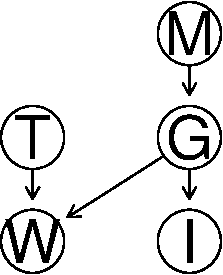
\includegraphics{BNfiles/unnamed-chunk-13-1} \end{center}

\noindent
 Note that the scenario node unifies the different events and states.
Because of this unifying role, increasing the probability of one part of
the scenario (say \textsf{State/event 2}) will also increase the
probability of the other parts (\textsf{State/event 1} and
\textsf{State/event 3}). This is intended to capture the idea that the
different components of a scenario form an interconnected sequence of
events.

One challenge that this strategy is supposed to help with is the
question of how to make sense of the notion of the coherence of a
scenario as different from its probability given the evidence. On this
approach (Vlek, 2016; Vlek, Prakken, Renooij, \& Bart Verheij, 2015;
Vlek, Prakken, Renooij, \& Verheij, 2013; Vlek et al., 2014), coherence
is identified with the prior probability of the scenario node.

Another challenge that the framework is supossed to meet is the question
of how to formally represent reasoning with multiple scenarios on the
table. On this approach (called scenario merging), given a class of
narrations, all the nodes used in some of the separate BNs are to be
used to build one large BN, and separate scenario nodes are to be added
to it, so that one BN supposedly represents multiple scenarios at once.

A somewhat alternative approach to representation of and reasoning with
multiple scenarios has been developed by Neil, Fenton, Lagnado, \& Gill
(2019). They correctly criticize (Urbaniak, 2018a) where I only sketch
some theoretical moves in a second-order language towards the
probabilistic modelling of the narrative approach. The critics point out
the paper makes no connection to BNs and so it ``fails to offer a
convincing and operational means to structure and compare competing
narratives.'' This is a fair assessment of the limits of what I have
achieved so far. They propose to represent separate narrations in terms
of separate BNs, and to deploy bayesian model comparison and averaging
as a tool for reasoning with multiple scenarios. That is, Bayes Theorem
with hypotheses as models (BNs), yields:

\vspace{-3mm}

\begin{align}
\pr{M=m_i\vert E} & = \frac{
\pr{E\vert M = m_i}\pr{M= m_i}
}
{
\sum_{i=1}^{n}\pr{E \vert M = m_i}\pr{M = m_i}
}
\end{align}

\noindent Then, assuming equal priors, models with higher likelihoods
will have higher posterior probabilities, and the most plausible model
will be the one with the highest posterior (that is, with equal priors,
with highest likelihood). Alternatively, they propose averaging the
predictions for a given variable \(\varphi\) by taking the ensemble
model:

\vspace{-3mm}

\begin{align}
\pr{\varphi \vert E} & = \sum_{i=1}^n \pr{\varphi \vert M=m_i, E} \pr{M=m_i\vert E}
\end{align}

\vspace{-2mm}

\noindent where the priors are either equal or are identified with the
posterior of the models given the evidence, and those posteriors are to
be calculated assuming equal priors.

\subsection{Pioneering nature of the
project}\label{pioneering-nature-of-the-project}

\subsubsection{Points of disagreement}\label{points-of-disagreement}

Here are the key reasons why I am convinced the scenario node approach
is not satisfactory:

\begin{enumerate}
\def\labelenumi{\Alph{enumi}.}
\item
  The use of a scenario idiom is problematic. Adding a parent node by
  \emph{fiat} without any good reasons to think the nodes are connected
  other than being a part of a single story, introduces probabilistic
  dependencies between the elements of a narration. Merely saying that,
  say, the defenendant made jointly some claims is not a good reason to
  assume they are probabilistically dependent.
\item
  Another problem results from the identification of prior probability
  with coherence. This does not add up intuitively. After all, it is
  quite coherent with my views that if I win a lottery, I'll buy a large
  house in Auckland and move there, while both the prior and the
  posterior given the total available evidence of this scenario are
  rather low.
\item
  In general, the legal probabilistic approach to coherence is very
  simple and fails to engage with rich philosophical literature exactly
  on this topic (Douven \& Meijs, 2007; Fitelson, 2003a, 2003b; Glass,
  2002; Meijs \& Douven, 2007; Olsson, 2001; Shogenji, 1999), including
  a long list of counterexamples to the existing proposals and
  desiderata that a probabilistic coherence measure should satisfy
  (Akiba, 2000; Bovens \& Hartmann, 2004; Crupi, Tentori, \& Gonzalez,
  2007; Koscholke, 2016; Merricks, 1995; Schippers \& Koscholke, 2019;
  Shogenji, 1999, 2001, 2006; Siebel, 2004, 2006).
\item
  The merging procedure with scenario nodes assumes that for the nodes
  that are common to the networks to be merged, both the directions of
  the arrows in the DAGs and the conditional probability tables are the
  same across different narrations. This is suboptimal. Different sides
  in court might construe causal dependencies differently, and even if
  they agree about the direction of an arrow, they might disagree about
  the probability table associated with it. Even a single side might
  consider different scenarios with different probabilities, say, when
  there is some uncertaintly inolved in the probability assignment
  itself.
\end{enumerate}

\vspace{2mm}

Here are the key limitations of the approach proposed by Neil et al.
(2019):

\begin{enumerate}
\def\labelenumi{\Alph{enumi}.}
\setcounter{enumi}{4}
\item
  The assumption of equal priors is highly debatable. For one thing,
  this approach would render prior probabilities quite sensitive to the
  choice of hypotheses and thus potentially arbitrary. In addition, this
  approach seems particularly unsuitable for criminal cases. If the only
  two hypotheses/models on the table ultimately say ``the defendant is
  guilty'' and ``the defendant is innocent'', the prior probability of
  each would be 50\%. But defendants in criminal cases, however, should
  be presumed innocent until proven guilty. A 50\% prior probability of
  guilt seems excessive. Some (Williamson, 2010) try to defend a variant
  of the principle of indifference by reference to informational
  entropy, and a proposal along this line has been used in practical
  recommendation by expert committees (ENFSI Expert Working Group Marks
  Conclusion Scale Committee, 2006). However, this attempt has been
  sensibly criticized by Biedermann, Taroni, \& Garbolino (2007). The
  question remains, what should the proper application of informational
  entropy in the context of BN selection and averaging look like, given
  that information entropy considerations independently are in
  epistemologically decent standing? Importantly, whatever conclusions
  in such contexts are epistemologically justified, how do they square
  with the presumption of innocence? Some take the presumption to mean
  that the prior probability of guilt should be set to a small value
  (Friedman, 2000; Friedman, Allen, Balding, Donnelly, \& Kaye, 1995),
  but it is not clear whether this interpretation can be justified on
  epistemological or decision-theoretic grounds.
\item
  More recent models rely on relevant background information, for
  example, geographical information about people's opportunities to
  commit crimes {[}Fenton, Lagnado, Dahlman, \& Neil (2019). But even if
  these models are successful in giving well-informed assessments of
  prior probabilities any evidence-based assessment of prior
  probabilities, they are likely to violate existing normative
  requirements of the trial system (Dahlman, 2017; Engel, 2012;
  Schweizer, 2013). For instance, if the assessment of prior
  probabilities relies on demographic information, people who belong to
  certain demographic groups will be regarded as having a higher prior
  probability of committing a wrong than others. This is what a
  well-informed assessment should amount to. Yet, if some people's
  priors are higher than other people's priors, it will be easier to
  convict or find liable those who are assigned higher priors, even if
  the evidence against them is the same as the evidence against those
  assigned lower priors. This outcome can be seen as unfair (Di Bello \&
  O'Neil, 2020). The question remains: what procedure of choosing the
  priors both is justified by epistemological considerations and does
  not generate tension with fairness considerations?
\item
  Model selection based on likelihood (given equal priors) or posterior
  model probabilities in general (if priors are not assumed to be equal)
  boils down to a variant of the threshold view, and so all the
  difficulties with the threshold view apply.
\item
  Model averaging in the proposed form boils down to taking a weighted
  average of the probabilities provided by the models (weighted linear
  pooling). However, there is a rich literature on the difficulties that
  linear pooling runs into (see the surveys in Dietrich \& List, 2016;
  Franz Dietrich \& List, 2017a, 2017b). One problem is that the method
  satisfies the unanimity assumption: whenever all models share a degree
  of belief in a claim, this is exactly the output degree for that
  belief. But clearly, a claim can receive additional boost from
  multiple agents with different pieces of evidence agreeing on
  something (for instance, in witness corroboration). Another problem is
  that linear pooling does not preserve probabilistic independence (List
  \& Pettit, 2011): even if all models agree that certain nodes are
  independent, they might end up being dependent in the output. There is
  also a variety of impossibility theorems in the neighborhood (Gallow,
  2018).\textbackslash{}footnote\{Here is a nice example. It turns out
  you can't at the same time hold the following:

  \begin{align}
  \pr{A=B} & <1\\
  \pr{r\vert A=a} & = a \\
  \pr{r\vert B=b} & = b \\
  \forall a,b \, \pr{r \vert A =a, B = b} & =  \alpha a + \beta b
  \end{align}
\end{enumerate}

\noindent This means that that it is impossible that two models \(A\)
and \(B\) can disagree, we trust each of them separately if we only
learn about one model, and we take a weighted average if we learn about
both.\}

\subsubsection{Strategy and novelty}\label{strategy-and-novelty}

First, we need to represent narrations with their argumentative and
dynamic structure in probabilistic terms. Once this is done, the
resulting rich structure can be used to work out a better explication of
the notion of coherence. Once this is done, various methods of dealing
with multiple BNs, be it ensemble methods or some model selection
methods, should be put into place, by explaining in a principled way
which of these methods should be used in what context and why. One key
novelty is in the formulation and BN implementation of selection
criteria that so far have only been discussed informally in
philosophical literature. Once this explication is obtained, further
investigation of the role these criteria should play and their
principled justification will proceed. I cover these steps in more
detail now.

\noindent
\textbf{Representation.} I will use BNs taken separately without
scenario nodes to represent various narrations. Crucially, I will not
assume the conditional probability tables or directions of edges are the
same across the BNs, thus allowing for more realistic flexibility. To be
able to accommodate insights provided by NPAS and other critics of LP, I
will add another layer of information: for each BN one needs to specify
a set of binary nodes such that a certain combination of their states
counts as a narration, and a set of evidence nodes, which are supposed
to support this narration.

\noindent \textbf{Dynamic BNs} If what we are modeling is
cross-examination, averaging does not seem to be the right way to go. To
model cross-examination, we need to take the argumentative approach
seriously and to be able to model relations such as ``undercutting'' and
``rebutting''. And these relations can be modelled by adding or removing
nodes or arrows in the network in a suitable manner. But this means we
might have to consider another dimension: BNs changing through time in
light of other BNs. How to make sense of this formally so that the
result makes sense philosophically remains an open question.

\noindent
 \textbf{BN-based coherence.} I have developed a coherence measure that
diverges from the known candidates in three important respects: (1) It
is not a function of a probabilistic measure and a set of propositions
alone, because it is also sensitive to the selection and direction of
arrows in a Bayesian Network representing an agent's credal state. (2)
Unlike in the case of quite a few coherence measures, it is not obtained
by taking a mean of some list of intermediate values (such as
confirmation levels between subsets of a narration). It is sensitive
also to the variance and the minimal values of the intermediate values.
(3) The intermediate values used are not confirmation levels, but rather
expected and weighted confirmation levels. Preliminary tests on existing
philosophical counterexamples suggests the performance of the measure is
much better than the existing coherence measures. Now, it needs to be
deployed (implemented in \textbf{\textsf{R}} for BNs) and properly
tested on real-life cases discussed in the LP literature.

\noindent
 \textbf{Divide and conquer.} In fact, dealing with multiple models is
difficult in this context. On one hand, many machine learning methods
are not available. For instance, one cannot evaluate models in terms of
their performance with respect to the data. Whenever you want to use
resampling methods (such as cross-validation), or some information
criterion scoring (suchs as Akaike Information Criterion), you need to
have a dataset with multiple datapoints to start with, and such datasets
are usually not available (and often conceptually unimaginable) for the
problems typically faced in the court of law. On the other hand,
averaging often doesn't make sense either. After all, often no
epistemological or decision-related progress might be gained based on
averaging the prosecutor's and the defendant's stories. I propose that
ensemble methods should be deployed for multiple narration variants
available from one side (as in when, say, the prosecution story comes
with uncertainty about the direction of an arrow or about a particular
probability table), but selection methods should be used when final
decision is to be made between narrations proposed by the opposing
sides.

\noindent
\textbf{Ensemble methods.} One question that arises is whether the
general concerns about linear pooling arise for such limited
applications. If not, the remaining concern is what priors should be
used. In light of the controversial nature of equal priors, I plan to
study the consequences of rescaling coherence scores (already mentioned)
to constitute model priors. The idea is that given that narrations are
to be developed by the sides themselves, taking coherence of their
narration as determining the prior might be more fair than using equal
priors or relying on geographical or population statistics. If yes,
perhaps some other methods boiling down to a variant of sensitivity
analysis can be deployed: look at all BNs corresponding to some variant
of the narration of one of the sides, find the strongest and the weakest
one, and these give you a range of possible outcomes.

\noindent
 \textbf{Selection criteria.} The so-called New Legal Probabilism (NLP)
is an attempt to improve on the underspecificity of NPAS (Di Bello,
2013). While still being at most semi-formal, the approach is more
specific about the conditions that a successful accusing narration is to
satisfy for the conviction beyond reasonable doubt to be justified. Di
Bello identifies four key requirements that a successful convicting
narration should satisfy:

\vspace{2mm}

\begin{center}
\begin{tabular}{@{}lp{11.5cm}@{}}
\toprule
 (Evidential support) &The defendant's guilt probability on the evidence should be sufficiently supported by the evidence, and a successful accusing narration should explain the relevant evidence. \\
(Evidential completeness) &  The evidence available at trial should be complete as far as a reasonable fact-finders' expectations are concerned. \\
(Resiliency)&  The prosecutor's narrative, based on the available evidence, should not be susceptible to revision given reasonably possible future arguments and evidence. \\
(Narrativity) & The narrative offered by the prosecutor should answer all 
the natural or reasonable questions one may have about what happened, given the content of the prosecutor's narration and the available evidence. \\
\bottomrule
\end{tabular}
\end{center}

\vspace{2mm}

\emph{Prima facie,} it is far from obvious that such conditions are
susceptible to a Bayesian networks explication. However, I have already
developed a more expressive probabilistic framework (call it
Narration-Friendly Probabilism (NFP)) capable of expressing such
features within a formalized higher-order language (Urbaniak, 2018b). On
NFP, the notion of narration is quite wide: narrations not only contain
factual statements about what happened, but also claims about evidence,
about narrations, about relations between evidence and various parts of
various narrations etc. I extend the basic propositional language with
propositional operators \(N_i\) and \(E\) corresponding to
``\emph{\dots is part of narration $i$}'' and
``\emph{\dots is part of the evidence},'' and model narrations as finite
sets of sentences from this language. Due to this intuitive move, many
important aspects of narrations normally discussed only informally,
similar to those discussed by Di Bello, become expressible in terms of
probabilistic measures for such a formal language. Let's very briefly
gesture towards a few examples:

\begin{itemize}\setlength\itemsep{-1mm}
 \item A defending narration explains  a piece of evidence  $e$ just in case  if there is an  attacking narration whose posterior is raised conditional on $e$, the probability of $e$ conditional on this defending narration is above the negligibility threshold.
 \item An attacking narration misses some evidence just in case there are some statements not in the evidence set such that the probability of the claim that at least one of them is part of evidence conditional on the existing evidence ($\{\varphi\vert \varphi \in \mbox{ Evidence}\}$), its description ($\{E\varphi\vert \varphi \in \mbox{ Evidence}\}$), and on this attacking narration is above the strong plausibility threshold. 
 \item A narration contains gaps just in case there are some claims which are not part of it, but conditional on the content and the description of this narration and the evidence available, their disjunction is strongly plausible, and it is strongly plausible conditional on the content (but not on the description) of this narration and on evidence that at least one of these claims is part of the narration.
 \item  A narration is dominant just in case it doesn't miss any evidence, it doesn’t contain any gap, and in light of all available information and evidence it is at least as likely any other accusing narration, and is strongly plausible.
 \end{itemize}

While threshold- or likelihood-ratio-based selection criteria for models
are unlikely to succeed, as already discussed, I am convinced the
criteria formulated in philosophical terms in (Di Bello, 2013) and in
higher-order terms in (Urbaniak, 2018a) are in better standing. The key
hypothesis is that they can be recast in terms of properties of BNs and
that the existing BN programming tools can be extended to implement
testing for these criteria. This will make them susceptible to
programmatic implementation and further study by means of computational
methods. The hope is that on one hand, they will do better than the
existing proposals, and where they fail, further insights can be gained
by studying the reasons behind such failures.

\section{Work plan}\label{work-plan}

\vspace{1mm}

\begin{center}
\begin{tabular}{p{2.3cm}|p{12.2cm}}
\footnotesize \textbf{$\mathtt{Stage  \,\, 1}$} \newline  \tiny Philosophical \&  formal \newline  unification & 
Obtain a unifying extended  probabilistic framework by incorporating further insights  from philosophical and psychological accounts of legal narrations, and from the argumentation approach. Defend its philosophical plausibility. \scriptsize (6 months)
\\
\footnotesize \textbf{$\mathtt{Stage \,\, 2}$} \newline  \tiny AI implementation 
 & Develop Bayesian Network Methods for the obtained formal framework, so that the insights from the argumentation approach and informal epistemology, mediated through it, can be incorporated in AI tools. \scriptsize (12 months)
\\
\footnotesize \textbf{$\mathtt{Stage  \,\, 3}$} \newline  \tiny    Case studies & 
Evaluate the developed framework and AI tools  by conducting case studies from its perspective.    \scriptsize (6 months) 
\\
\footnotesize \textbf{$\mathtt{Stage  \,\, 4}$} \newline  \tiny    Back to challenges \& output & 
Investigate the extent to which the new framework helps to handle the issues raised in points A.-H., finalize the book. \scriptsize (12 months)
\end{tabular}
\end{center}

\vspace{2mm}

The planned publication output is as follows:

\begin{itemize}\setlength\itemsep{1mm}
\item \textsf{Stage 1} will result in  one philosophical paper published in an  academic journal such as \emph{Synthese}, \emph{Mind} or \emph{Ratio Juris}. Working title: \emph{Why care about narration selection principles?}

\item \textsf{Stage 2} will lead to one   technical paper  published in a journal such as \emph{IfCoLog Journal of Logics and their Applications}, \emph{Law, Probability and Risk} or \emph{Artificial Intelligence and Law}. Working title: \emph{Implementation of narration assessment criteria in Bayesian Networks with \textbf{\textsf{R}}}.

\item \textsf{Stage 3}  will lead to a publication of one paper  on  how the formal framework handles case studies and  a further paper  on how the developed AI tools handle real-life situations in   journals such as \emph{Artificial Intelligence} or \emph{Argument \& Computation}. Working titles: \emph{Rethinking the famous BN-modeled cases within the narration framework} and \emph{BNarr, an \textbf{\textsf{R}} package to model narrations with Bayesian Networks}.

\item Throughout the  whole project I plan to cooperate with Marcello Di Bello. Over the last year we co-authored the Stanford Encyclopedia of Philosophy entry on Legal Probabilism. We decided to continue our fruitful cooperation. For over two months we have been working on a book proposal to be submitted to Oxford University Press exactly on the issues to be studied in this research project. Marcello Di Bello is an excellent philsopher with extensive research experience in the philosophy of legal evidence, and he would bring his expertise to the table when working both on the book and on the papers, whereas I would be focused on the technical aspects and the underlying  formal philosophy. During the last year of the research \textbf{I plan a six months' stay at Arizona University}, to work in person with Di Bello on finalizing the book that presents the results with special focus on issues investigated in \textsf{Stage 4}.
\end{itemize}

\pagebreak 

The tentative list of planned chapters is as follows (two of them
already exist as sample chapters for the book proposal submission):

\renewcommand{\labelenumi}{\Roman{enumi}}
\renewcommand{\labelenumii}{\arabic{enumii}}
\renewcommand{\labelenumiii}{\arabic{enumii}.\arabic{enumiii}}

\begin{multicols}{2}
\footnotesize
\begin{enumerate}
\item Legal probabilism and its foes
\begin{enumerate}

  \item The emergence of legal probabilism
  \begin{enumerate}
  \item  Famous cases
  \item  Probabilistic evidence
  \item  Trial by mathematics
  \item  Some history
  \end{enumerate}

  \item  A skeptical perspective
  \begin{enumerate}
  \item The difficulty about conjunction
  \item The complexity objection
  \item  The problem of corroboration
  \item  The problem of artificial precision
  \item Naked statistical evidence
  \item  The problem of priors
  \item  The reference class problem
  \item  Non-probabilistic perspectives
  \end{enumerate}


\end{enumerate}
\item  Evidence assessment
\begin{enumerate}


\setcounter{enumii}{2}
  \item  Bayes' Theorem and the usual fallacies
  \begin{enumerate}
  \item  Assuming independence
  \item  The prosecutor's fallacy
  \item  Base rate fallacy
  \item  Defense attorney's fallacy
  \item  Uniqueness fallacy
  \item  Case studies
  \end{enumerate}

  \item  Complications and caveats
  \begin{enumerate}
  \item  Complex hypotheses and complex bodies of evidence
  \item Source, activity and offense level hypotheses
  \item  Where do the numbers come from?
  \item  Modeling corroboration
  \item  Stories, explanations and coherence
  \end{enumerate}

  \item  Likelihood Ratios and Relevance
  \begin{enumerate}
  \item Likelihood ratio as a measure of evidence strength
  \item The risk of false positive and its impact
  \item Hypothesis choice
  \item Levels of hypotheses and the two-stain problem
  \item Relevance and the small-town murder scenario
  \item The cold-hit confusion
  \item  Likelihood ratio and  cold-hit DNA matches
  \end{enumerate}



  \item  Bayesian Networks
  \begin{enumerate}
  \item  Bayesian networks to the rescue
  \item  Legal evidence idioms
  \item Scenario idioms
  \item Modeling relevance
  \item  Case study: Sally Clark
  \item DNA evidence
  \end{enumerate}
  
  \item Corroboration
  \begin{enumerate}
  \item Boole's formula and Cohen's challenge
  \item  Modeling substantial rise in case of agreement
  \item Ekel\"of's corroboration measure and evidentiary mechanisms
  \item General approach with multiple false stories and multiple witnesses
  \end{enumerate}

  \item Coherence
  \begin{enumerate}
  \item  Existing probabilistic coherence measures
  \item  An array of counterexamples
  \item Coherence of structured narrations with Bayesian networks
  \item  Application to legal cases
  \end{enumerate}

  \item  New legal probabilism
    \begin{enumerate}
    \item  Desiderata
    \item  A probabilistic framework for narrations
    \item  Probabilistic explications of the desiderata
    \item  Bayesian network implementation
    \end{enumerate}


\end{enumerate}
\item  Trial Decisions
\begin{enumerate}



\setcounter{enumii}{9}
  \item  The functions of the proof standards
  \begin{enumerate}
  \item  Conceptual desiderata
  \item  Protecting defendants
  \item  Error reduction and error distribution/allocation
  \item  Dispute resolution and public deference
  \item  Justification and answerability
  \end{enumerate}



  \item  Standards of proof
  \begin{enumerate}
  \item  Legal background
  \item  Probabilistic thresholds
  \item  Theoretical challenges
  \item  Specific narratives
  \item The comparative strategy
  \item  The likelihood strategy
  \item Challenges (again)
  \item Probabilistic thresholds revised
  \item  Bayesian networks and probabilistic standard of proof
  \end{enumerate}

  \item  Accuracy and the risk of error
  \begin{enumerate}
  \item  Minimizing expected costs
  \item  Minimizing expected errors
  \item  Expected v.\ actual errors
  \item  Competing accounts of the risk of error
  \item  Bayesian networks and the risk of error
  \end{enumerate}



  \item  Fairness in trial decisions
  \begin{enumerate}
  \item  Procedural v.\ substantive fairness
  \item  Competing measures of substantive fairness
  \item  Bayesian networks and fairnesss
  \end{enumerate}


  \item  Alternative accounts and legal probabilism
  \begin{enumerate}
  \item  Baconian probability
  \item  Relative Plausibility
  \item  Arguments
  \item  Sensitivity
  \item  Normic Support
  \item  Justification/foundherentism
  \item  Completeness
  \item  Relevant alternatives
  \item  Knowledge
  \end{enumerate}

\item Conclusions
\end{enumerate}
\end{enumerate}
\normalsize
\end{multicols}

Apart from publications, the results will be presented at various
conferences devoted to legal reasoning. These include the yearly
conferences of the
\emph{International Association for Artificial Intelligence and Law} and
of the \emph{Foundation for Legal Knowledge Based Systems (JURIX)}, and
more general conferences gathering formal philosophers, so that the
research is inspired by interaction not only with legal evidence
scholars, computer scientists, but also philosophers. I am also already
an invited speaker at the upcoming ``Probability and Proof'' conference
that will be part of an international conference on the philosophy of
legal evidence (``The Michele Taruffo Girona Evidence Week'') in Girona
(Spain) May 23-27 2022.

\section{Methodology}\label{methodology}

Standard arguments for the legitimacy of Bayesianism\footnote{See for
  example (Earman, 1992; Urbach \& Howson, 1993) for an early yet fairly
  comprehensive survey, or (Pettigrew, 2011) for a discussion of more
  recent contributions. See also (Bovens \& Hartmann, 2004; Bradley,
  2015; Swinburne, 2001).} deploy usually rather abstract pieces of
reasoning to the effect that if one's degrees of beliefs satisfy certain
conditions, they also have to satisfy the probabilistic requirements. My
approach to thinking about the plausibility of Bayesian epistemology is
rather unlike such approaches. Instead, I prefer the
\emph{proof-of-the-pudding} methodology. I am convinced that an
important part of the philosophical assessment of the Bayesian research
program has to do with its achievements or failures in contributing to
debates in philosophy which are not themselves debates about the status
of Bayesianism itself. In particular, it would be great news if insights
from Bayesian epistemology could be used to further development of
forensic AI and deepening our understanding of judiciary decision
making.

What the project will uniquely bring to the table is joining the
familiarity with epistemological debates on the nature of coherence
(which legal probabilists like Vlek or Fenton ignore or are unaware of),
familiarity with the details of evidence assessment in legal cases
(which formal epistemologists such as Fitelson ignore) and technical
skill to programmatically implement, simulate and test various
theoretical moves.

I will be using four methods: (a) informal conceptual analysis; (b)
formal conceptual analysis; (c) computational metods (R simulations,
etc.); and (d) case studies. I will rethink and model the existing
impliementations of whole-case-scale-BNs in legal evidence from the
perspective of the new framework and reconstruct cases which extensively
use probabilistic reasoning, but for which BNs have not been yet
proposed. Both the literature already listed and many textbooks on
quantitative evidence in forensics are great sources of such cases.

A larger initiative involving reconstructing various cases using
different representation methods and comparing the representations,
called \emph{Probability and statistics in forensic science}, took place
at the Isaac Newton Institute for Mathematical Sciences. My approach
will be in the same vein.

I have extensive experience in analytic philosophy, conceptual analysis,
philosophical logic and probabilistic and decision-theoretic methods as
deployed in philosophical contexts. I also have teaching and publishing
record that involves statistical programming in the \textsf{\textbf{R}}
language (my sample programming projects can be visited at
\url{https://rfl-urbaniak.github.io/menu/projects.html}), and so am also
competent to develop AI implementations and tests of the ideas to be
developed.

One research risk is that it will turn out that some of the informal
requirements cannot be spelled out in probabilistic terms, or expressed
in terms of properties of Bayesian networks. In such an event, I will
study the reasons for this negative result. It might happen that there
are independent reasons to abandoned a given condition, or it might be
the case that probabilistic inexplicability of a given condition is an
argument against the probabilistic approach. Either way, finding out
which option holds and why would also lead to a deeper understanding of
the framework and lead to a publication in academic journals. Another
research risk is that the case studies will show that other methods are
more efficient or transparent. This would itself constitute a result
that could be used to further modify the framework so that its best
aspects could be preserved, while the disadvantages discovered during
case studies avoided.

\section{References}\label{references}

\footnotesize 

\hypertarget{refs}{}
\hypertarget{ref-Akiba2000Shogenjis}{}
Akiba, K. (2000). Shogenji's probabilistic measure of coherence is
incoherent. \emph{Analysis}, \emph{60}(4), 356--359. Oxford University
Press (OUP). Retrieved from
\url{https://doi.org/10.1093/analys/60.4.356}

\hypertarget{ref-Allen1986A-Reconceptuali}{}
Allen, R. J. (1986). A reconceptualization of civil trials. \emph{Boston
University Law Review}, \emph{66}, 401--437.

\hypertarget{ref-Allen2010No-Plausible-Al}{}
Allen, R. J. (2010). No plausible alternative to a plausible story of
guilt as the rule of decision in criminal cases. In J. Cruz \& L. Laudan
(Eds.), \emph{Prueba y esandares de prueba en el derecho}. Instituto de
Investigaciones Filosoficas-UNAM.

\hypertarget{ref-allen2001naturalized}{}
Allen, R. J., \& Leiter, B. (2001). Naturalized epistemology and the law
of evidence. \emph{Virginia Law Review}, \emph{87}(8), 1491--1550.
JSTOR.

\hypertarget{ref-allen2007problematic}{}
Allen, R., \& Pardo, M. (2007). The problematic value of mathematical
models of evidence. \emph{The Journal of Legal Studies}, \emph{36}(1),
107--140. JSTOR.

\hypertarget{ref-becker1968crime}{}
Becker, G. S. (1968). Crime and punishment: An economic approach.
\emph{Journal of Political Economy}, \emph{76}, 169--217. Springer.

\hypertarget{ref-Bernoulli1713Ars-conjectandi}{}
Bernoulli, J. (1713). \emph{Ars conjectandi}.

\hypertarget{ref-bex2015IntegratedTheoryCausal}{}
Bex, F. (2015). An integrated theory of causal stories and evidential
arguments. In \emph{Proceedings of the 15th International Conference on
Artificial Intelligence and Law - ICAIL '15} (pp. 13--22). San Diego,
California: ACM Press.

\hypertarget{ref-bex2011ArgumentsStoriesCriminal}{}
Bex, F. J. (2011). \emph{Arguments, stories and criminal evidence: A
formal hybrid theory}. Law and philosophy library. Dordrecht ; New York:
Springer.

\hypertarget{ref-Biedermann2007equal}{}
Biedermann, A., Taroni, F., \& Garbolino, P. (2007). Equal prior
probabilities: Can one do any better? \emph{Forensic Science
International}, \emph{172}(2-3), 85--93. Elsevier BV. Retrieved from
\url{https://doi.org/10.1016/j.forsciint.2006.12.008}

\hypertarget{ref-bovens2004bayesian}{}
Bovens, L., \& Hartmann, S. (2004). \emph{Bayesian epistemology}. Oxford
University Press.

\hypertarget{ref-bradley2015critical}{}
Bradley, D. (2015). \emph{A critical introduction to formal
epistemology}. Bloomsbury Publishing.

\hypertarget{ref-brilmayer1986}{}
Brilmayer, L. (1986). Second-order evidence and bayesian logic.
\emph{Boston University Law Review}, \emph{66}, 673--691.

\hypertarget{ref-Calabresi1961}{}
Calabresi, G. (1961). Some thoughts on risk distribution and the law of
torts. \emph{Yale Law Journal}, \emph{70}, 499--553.

\hypertarget{ref-clermont2015TrialTraditionalProbability}{}
Clermont, K. M. (2015). Trial by Traditional Probability, Relative
Plausibility, or Belief Function? \emph{Case Western Reserve Law
Review}, \emph{66}(2), 353--391.

\hypertarget{ref-Cohen81}{}
Cohen, J. L. (1981). Subjective probability and the paradox of the
Gatecrasher. \emph{Arizona State Law Journal}, 627--634.

\hypertarget{ref-cohen86}{}
Cohen, J. L. (1986). Twelve questions about Keynes's concept of weight.
\emph{British Journal for the Philosophy of Science}, \emph{37}(3),
263--278.

\hypertarget{ref-crupi2007BayesianMeasuresEvidential}{}
Crupi, V., Tentori, K., \& Gonzalez, M. (2007). On Bayesian Measures of
Evidential Support: Theoretical and Empirical Issues. \emph{Philosophy
of Science}, \emph{74}(2), 229--252.

\hypertarget{ref-dahlman2017}{}
Dahlman, C. (2017). Determining the base rate for guilt. \emph{Law,
Probability and Risk}, \emph{17}(1), 15--28.

\hypertarget{ref-dant1988gambling}{}
Dant, M. (1988). Gambling on the truth: The use of purely statistical
evidence as a basis for civil liability. \emph{Columbia Journal of Law
and Social Problems}, \emph{22}, 31--70. HeinOnline.

\hypertarget{ref-daston1988}{}
Daston, L. (1988). \emph{Classical probability in the enlightenment}.
Princeton University Press.

\hypertarget{ref-dawid2018graphical}{}
Dawid, A. P., \& Mortera, J. (2018). Graphical models for forensic
analysis. In \emph{Handbook of graphical models} (pp. 491--514). CRC
Press.

\hypertarget{ref-Dekay1996}{}
Dekay, M. L. (1996). The difference between Blackstone-like error ratios
and probabilistic standards of proof. \emph{Law and Social Inquiry},
\emph{21}, 95--132.

\hypertarget{ref-di2013statistics}{}
Di Bello, M. (2013). \emph{Statistics and probability in criminal
trials} (PhD thesis). University of Stanford.

\hypertarget{ref-DiBelloONeil2020}{}
Di Bello, M., \& O'Neil, C. (2020). Profile evidence, fairness and the
risk of mistaken convictions. \emph{Ethics}, \emph{130}(2), 147--178.

\hypertarget{ref-di2018evidential}{}
Di Bello, M., \& Verheij, B. (2018). Evidential reasoning. In
\emph{Handbook of legal reasoning and argumentation} (pp. 447--493).
Springer.

\hypertarget{ref-diamond90}{}
Diamond, H. A. (1990). Reasonable doubt: To define, or not to define.
\emph{Columbia Law Review}, \emph{90}(6), 1716--1736.

\hypertarget{ref-Dietrich2016Probabilistic}{}
Dietrich, F., \& List, C. (2016). Probabilistic opinion pooling. In A.
Hajek \& C. Hitchcock (Eds.), \emph{Oxford handbook of philosophy and
probability}. Oxford University Press.

\hypertarget{ref-dietrich2017probabilistic1}{}
Dietrich, F., \& List, C. (2017a). Probabilistic opinion pooling
generalized. part one: General agendas. \emph{Social Choice and
Welfare}, \emph{48}(4), 747--786. Springer.

\hypertarget{ref-dietrich2017probabilistic2}{}
Dietrich, F., \& List, C. (2017b). Probabilistic opinion pooling
generalized. part two: The premise-based approach. \emph{Social Choice
and Welfare}, \emph{48}(4), 787--814. Springer.

\hypertarget{ref-Douven2007measuring}{}
Douven, I., \& Meijs, W. (2007). Measuring coherence. \emph{Synthese},
\emph{156}(3), 405--425. Springer Science; Business Media LLC. Retrieved
from \url{https://doi.org/10.1007/s11229-006-9131-z}

\hypertarget{ref-earman1992bayes}{}
Earman, J. (1992). \emph{Bayes or bust? A critical examination of
bayesian confirmation theory}. Cambridge: MIT Press.

\hypertarget{ref-Edwards1991Influence-diagr}{}
Edwards, W. (1991). Influence diagrams, bayesian imperialism, and the
collins case: An appeal to reason. \emph{Cardozo Law Review}, \emph{13},
1025--1074.

\hypertarget{ref-ENFSI2006entropy}{}
ENFSI Expert Working Group Marks Conclusion Scale Committee. (2006).
Conclusion scale for shoeprint and toolmarks examinations. \emph{Journal
of Forensic Identification}, \emph{56}, 255--280.

\hypertarget{ref-engel2012NeglectBaseRate}{}
Engel, C. (2012). Neglect the Base Rate: It's the Law! \emph{Preprints
of the Max Planck Institute for Research on Collective Goods},
\emph{23}.

\hypertarget{ref-enoch2015sense}{}
Enoch, D., \& Fisher, T. (2015). Sense and sensitivity: Epistemic and
instrumental approaches to statistical evidence. \emph{Stan. L. Rev.},
\emph{67}, 557--611. HeinOnline.

\hypertarget{ref-Fenton2018risk}{}
Fenton, N., \& Neil, M. (2018a). \emph{Risk assessment and decision
analysis with Bayesian networks}. Chapman; Hall.

\hypertarget{ref-Fenton2018Risk}{}
Fenton, N., \& Neil, M. (2018b). \emph{Risk assessment and decision
analysis with bayesian networks}. Chapman; Hall.

\hypertarget{ref-fenton2019OpportunityPriorProofbased}{}
Fenton, N., Lagnado, D., Dahlman, C., \& Neil, M. (2019). The
opportunity prior: A proof-based prior for criminal cases. \emph{Law,
Probability and Risk}, {[}online first{]}.

\hypertarget{ref-fenton2013GeneralStructureLegal}{}
Fenton, N., Neil, M., \& Lagnado, D. A. (2013). A General Structure for
Legal Arguments About Evidence Using Bayesian Networks. \emph{Cognitive
Science}, \emph{37}(1), 61--102.

\hypertarget{ref-Finkelstein1970A}{}
Finkelstein, M. O., \& Fairley, W. B. (1970). A Bayesian approach to
identification evidence. \emph{Harvard Law Review}, \emph{83}(3),
489--517.

\hypertarget{ref-fitelson2003ProbabilisticTheoryCoherence}{}
Fitelson, B. (2003a). A Probabilistic Theory of Coherence.
\emph{Analysis}, \emph{63}(3), 194--199.

\hypertarget{ref-fitelson2003comments}{}
Fitelson, B. (2003b). Comments on jim franklin's the representation of
context: Ideas from artificial intelligence (or, more remarks on the
contextuality of probability). \emph{Law, Probability and Risk},
\emph{2}(3), 201--204. Oxford Univ Press.

\hypertarget{ref-Franklin2001}{}
Franklin, J. (2001). \emph{The science of conjecture: Evidence and
probability before pascal}. John Hopkins University Press.

\hypertarget{ref-friedman1974}{}
Friedman, M. (1974). Explanation and scientific understanding.
\emph{Journal of Philosophy}, \emph{71}, 5--19.

\hypertarget{ref-Friedman2000}{}
Friedman, R. D. (2000). A presumption of innocence, not of even odds.
\emph{Stanford Law Review}, \emph{52}(4), 873--887.

\hypertarget{ref-friedmanEtAl1995}{}
Friedman, R. D., Allen, R. J., Balding, D. J., Donnelly, P., \& Kaye, D.
H. (1995). Probability and proof in State v. Skipper: An internet
exchange. \emph{Jurimetrics}, \emph{35}(3), 277--310.

\hypertarget{ref-Gallow2018No}{}
Gallow, J. (2018). No one can serve two epistemic masters.
\emph{Philosophical Studies}, \emph{175}(10), 2389--2398. Springer
Verlag.

\hypertarget{ref-gardiner2018}{}
Gardiner, G. (2018). Legal burdens of proof and statistical evidence. In
D. Coady \& J. Chase (Eds.), \emph{Routledge handbook of applied
epistemology}. Routledge.

\hypertarget{ref-glass2002}{}
Glass, D. H. (2002). Coherence, Explanation, and Bayesian Networks. In
G. Goos, J. Hartmanis, J. van Leeuwen, M. O'Neill, R. F. E. Sutcliffe,
C. Ryan, M. Eaton, et al. (Eds.), \emph{Artificial Intelligence and
Cognitive Science} (Vol. 2464, pp. 177--182). Berlin, Heidelberg:
Springer Berlin Heidelberg.

\hypertarget{ref-gordon2007}{}
Gordon, T. F., Prakken, H., \& Walton, D. (2007). The Carneades model of
argument and burden of proof. \emph{Artificial Intelligence},
\emph{171}(10-15), 875--896.

\hypertarget{ref-haack2011legal}{}
Haack, S. (2014). Legal probabilism: An epistemological dissent. In
\emph{Haack2014-HAAEMS} (pp. 47--77).

\hypertarget{ref-Hacking1984}{}
Hacking, I. (1975). \emph{The emergence of probability: A philosophical
study of early ideas about probability, induction and statistical
inference}. Cambridge University Press.

\hypertarget{ref-hastie2019CaseRelativePlausibilitya}{}
Hastie, R. (2019). The case for relative plausibility theory: Promising,
but insufficient. \emph{The International Journal of Evidence \& Proof},
\emph{23}(1-2), 134--140.

\hypertarget{ref-hedden2019}{}
Hedden, B. (2019). Hindsight bias is not a bias. \emph{Analysis},
\emph{79}(1), 43--52.

\hypertarget{ref-hepler2007ObjectorientedGraphicalRepresentations}{}
Hepler, A. B., Dawid, A. P., \& Leucari, V. (2007). Object-oriented
graphical representations of complex patterns of evidence. \emph{Law,
Probability and Risk}, \emph{6}(1-4), 275--293.

\hypertarget{ref-ho2008philosophy}{}
Ho, H. L. (2008). \emph{A philosophy of evidence law: Justice in the
search for truth}. Oxford University Press.

\hypertarget{ref-lai2019HowPlausibleRelative}{}
Ho, H. L. (2019). How plausible is the relative plausibility theory of
proof? \emph{The International Journal of Evidence \& Proof},
\emph{23}(1-2), 191--197.

\hypertarget{ref-Horowitz1996}{}
Horowitz, I. A., \& Kirkpatrick, L. C. (1996). A concept in search of a
definition: The effect of reasonable doubt instrcutions on certainty of
guilt standards and jury verdicts. \emph{Law and Human Behaviour},
\emph{20}(6), 655--670.

\hypertarget{ref-kadane2011probabilistic}{}
Kadane, J. B., \& Schum, D. A. (2011). \emph{A probabilistic analysis of
the sacco and vanzetti evidence}. John Wiley \& Sons.

\hypertarget{ref-kaye79}{}
Kaye, D. H. (1979). The laws of probability and the law of the land.
\emph{The University of Chicago Law Review}, \emph{47}(1), 34--56.

\hypertarget{ref-kaye1986admissibility}{}
Kaye, D. H. (1986). The admissibility of ``probability evidence'' in
criminal trials---part I. \emph{Jurimetrics Journal}, 343--346.

\hypertarget{ref-Kaye2010The-Double-Heli}{}
Kaye, D. H. (2010). \emph{The double helix and the law of evidence}.
Harvard University Press.

\hypertarget{ref-Koehler1996On-Conveying-th}{}
Koehler, J. J. (1996). On conveying the probative value of DNA evidence:
Frequencies, likelihood ratios, and error rates. \emph{University of
Colorado law Review}, \emph{67}, 859--886.

\hypertarget{ref-koscholke2016evaluating}{}
Koscholke, J. (2016). Evaluating Test Cases for Probabilistic Measures
of Coherence. \emph{Erkenntnis}, \emph{81}(1), 155--181.

\hypertarget{ref-Laplace1814}{}
Laplace, P. (1814). \emph{Essai philosophique sur les probabilités}.

\hypertarget{ref-laudan2006truth}{}
Laudan, L. (2006). \emph{Truth, error, and criminal law: An essay in
legal epistemology}. Cambridge University Press.

\hypertarget{ref-lempert1977modeling}{}
Lempert, R. O. (1977). Modeling relevance. \emph{Michigan Law Review},
\emph{75}, 1021--1057. JSTOR.

\hypertarget{ref-Lempert1986}{}
Lempert, R. O. (1986). The new evidence scholarship: Analysing the
process of proof. \emph{Boston University Law Review}, \emph{66},
439--477.

\hypertarget{ref-Lipton2004-LIPITT}{}
Lipton, P. (2004). \emph{Inference to the best explanation}.
Routledge/Taylor; Francis Group.

\hypertarget{ref-List2011Group}{}
List, C., \& Pettit, P. (2011). \emph{Group agency: The possibility,
design, and status of corporate agents}. Oxford University Press.

\hypertarget{ref-lucy2013introduction}{}
Lucy, D. (2013). \emph{Introduction to statistics for forensic
scientists}. John Wiley \& Sons.

\hypertarget{ref-meijs2007}{}
Meijs, W., \& Douven, I. (2007). On the alleged impossibility of
coherence. \emph{Synthese}, \emph{157}(3), 347--360.

\hypertarget{ref-Merricks1995}{}
Merricks, T. (1995). Warrant entails truth. \emph{Philosophy and
Phenomenological Research}, \emph{55}, 841--855.

\hypertarget{ref-nance2019LimitationsRelativePlausibility}{}
Nance, D. A. (2019). The limitations of relative plausibility theory.
\emph{The International Journal of Evidence \& Proof}, \emph{23}(1-2),
154--160.

\hypertarget{ref-NRCI1992}{}
National Research Council. (1992). \emph{DNA technology in forensic
science \textup{{[}NRC I{]}}}. Committee on DNA technology in Forensic
Science, National Research Council.

\hypertarget{ref-neil2000BuildingLargescaleBayesian}{}
Neil, M., Fenton, N., \& Nielson, L. (2000). Building large-scale
Bayesian Networks. \emph{The Knowledge Engineering Review},
\emph{15}(3), 257--284.

\hypertarget{ref-Fenton2019Modelling}{}
Neil, M., Fenton, N., Lagnado, D., \& Gill, R. D. (2019). Modelling
competing legal arguments using bayesian model comparison and averaging.
\emph{Artificial Intelligence and Law}. Retrieved from
\url{https://doi.org/10.1007/s10506-019-09250-3}

\hypertarget{ref-Nesson1979Reasonable-doub}{}
Nesson, C. R. (1979). Reasonable doubt and permissive inferences: The
value of complexity. \emph{Harvard Law Review}, \emph{92}(6),
1187--1225.

\hypertarget{ref-newman1993}{}
Newman, J. O. (1993). Beyon ``reasonable doub''. \emph{New York
University Law Review}, \emph{68}(5), 979--1002.

\hypertarget{ref-olsson2001}{}
Olsson, E. J. (2001). Why Coherence Is Not Truth-Conducive.
\emph{Analysis}, \emph{61}(3), 236--241.

\hypertarget{ref-pardo2018}{}
Pardo, M. S. (2018). Safety vs.~Sensitivity: Possible worlds and the law
of evidence. \emph{Legal Theory}, \emph{24}(1), 50--75.

\hypertarget{ref-Pardo2008judicial}{}
Pardo, M. S., \& Allen, R. J. (2008). Judicial proof and the best
explanation. \emph{Law and Philosophy}, \emph{27}(3), 223--268.

\hypertarget{ref-Pennington1991}{}
Pennington, N., \& Hastie, R. (1991a). A cognitive theory of juror
decision making: The story model. \emph{Cardozo Law Review}, \emph{13},
519--557.

\hypertarget{ref-pennington1991cognitive}{}
Pennington, N., \& Hastie, R. (1991b). A cognitive theory of juror
decision making: The story model. \emph{Cardozo Law Review}, \emph{13},
519--557. HeinOnline.

\hypertarget{ref-pennington1992explaining}{}
Pennington, N., \& Hastie, R. (1992). Explaining the evidence: Tests of
the story model for juror decision making. \emph{Journal of personality
and social psychology}, \emph{62}(2), 189--204. American Psychological
Association.

\hypertarget{ref-Pettigrew2011Epistemic-Utili}{}
Pettigrew, R. (2011). Epistemic utility arguments for probabilism. In
\emph{Stanford encyclopedia of philosophy}.

\hypertarget{ref-Posner1973}{}
Posner, R. (1973). \emph{The economic analysis of law}. Brown \&
Company.

\hypertarget{ref-redmayne2008exploring}{}
Redmayne, M. (2008). Exploring the proof paradoxes. \emph{Legal Theory},
\emph{14}(4), 281--309. Cambridge University Press.

\hypertarget{ref-Robertson1995evidence}{}
Robertson, B., \& Vignaux, G. A. (1995). DNA evidence: Wrong answers or
wrong questions? \emph{Genetica}, \emph{96}, 145--152.

\hypertarget{ref-ross2020}{}
Ross, L. (2020). Rehabilitating statistical evidence. \emph{Philosophy
and Phenomenological Research}.

\hypertarget{ref-Schippers2019General}{}
Schippers, M., \& Koscholke, J. (2019). A General Framework for
Probabilistic Measures of Coherence. \emph{Studia Logica}.

\hypertarget{ref-schwartz2019WhatRelativePlausibility}{}
Schwartz, D. S., \& Sober, E. (2019). What is relative plausibility?
\emph{The International Journal of Evidence \& Proof}, \emph{23}(1-2),
198--204.

\hypertarget{ref-schweizer2013LawDoesnSay}{}
Schweizer, M. (2013). The Law Doesn't Say Much About Base Rates.
\emph{SSRN Electronic Journal}.

\hypertarget{ref-shen2007ScenariodrivenDecisionSupporta}{}
Shen, Q., Keppens, J., Aitken, C., Schafer, B., \& Lee, M. (2007). A
scenario-driven decision support system for serious crime investigation.
\emph{Law, Probability and Risk}, \emph{5}(2), 87--117.

\hypertarget{ref-shogenji1999}{}
Shogenji, T. (1999). Is Coherence Truth Conducive? \emph{Analysis},
\emph{59}(4), 338--345.

\hypertarget{ref-Shogenji2001Reply}{}
Shogenji, T. (2001). Reply to akiba on the probabilistic measure of
coherence. \emph{Analysis}, \emph{61}(2), 147--150. Oxford University
Press (OUP). Retrieved from
\url{https://doi.org/10.1093/analys/61.2.147}

\hypertarget{ref-Shogenji2006Why}{}
Shogenji, T. (2006). Why does coherence appear truth-conducive?
\emph{Synthese}, \emph{157}(3), 361--372. Springer Science; Business
Media LLC. Retrieved from
\url{https://doi.org/10.1007/s11229-006-9062-8}

\hypertarget{ref-Siebel2004On-Fitelsons-me}{}
Siebel, M. (2004). On Fitelson's measure of coherence. \emph{Analysis},
\emph{64}, 189--190.

\hypertarget{ref-siebel2006against}{}
Siebel, M. (2006). Against probabilistic measures of coherence. In
\emph{Coherence, truth and testimony} (pp. 43--68). Springer.

\hypertarget{ref-Smith_conviction_mind_2017}{}
Smith, M. (2017). When does evidence suffice for conviction?
\emph{Mind}.

\hypertarget{ref-Swinburne2001-SWIEJ}{}
Swinburne, R. (2001). \emph{Epistemic justification}. Oxford University
Press.

\hypertarget{ref-taroni2006bayesian}{}
Taroni, F., Biedermann, A., Bozza, S., Garbolino, P., \& Aitken, C.
(2014). \emph{Bayesian networks for probabilistic inference and decision
analysis in forensic science} (2nd ed.). John Wiley \& Sons.

\hypertarget{ref-Thomson86}{}
Thomson, J. J. (1986). Liability and individualized evidence. \emph{Law
and Contemporary Problems}, \emph{49}(3), 199--219.

\hypertarget{ref-tribe71}{}
Tribe, L. H. (1971). Trial by mathematics: Precision and ritual in the
legal process. \emph{Harvard Law Review}, \emph{84}(6), 1329--1393.

\hypertarget{ref-Underwood1977The-thumb-on-th}{}
Underwood, B. D. (1977). The thumb on the scale of justice: Burdens of
persuasion in criminal cases. \emph{Yale Law Journal}, \emph{86(7)},
1299--1348.

\hypertarget{ref-Urbach1993-HOWSRT}{}
Urbach, P., \& Howson, C. (1993). \emph{Scientific reasoning: The
bayesian approach}. Open Court.

\hypertarget{ref-urbaniak2018narration}{}
Urbaniak, R. (2018a). Narration in judiciary fact-finding: A
probabilistic explication. \emph{Artificial Intelligence and Law},
1--32.

\hypertarget{ref-Urbaniak2017Narration-in-ju}{}
Urbaniak, R. (2018b). Narration in judiciary fact-finding: A
probabilistic explication. \emph{Artificial Intelligence and Law},
1--32.

\hypertarget{ref-Urbaniak2020Decision}{}
Urbaniak, R., Kowalewska, A., Janda, P., \& Dziurosz-Serafinowicz, P.
(2020). Decision-theoretic and risk-based approaches to naked
statistical evidence: Some consequences and challenges. \emph{Law,
Probability and Risk}.

\hypertarget{ref-vanEemeren2017}{}
van Eemeren, F., \& Verheij, B. (2017). Argumentation theory in formal
and computational perspective. \emph{IFCoLog Journal of Logics and Their
Applications}, \emph{4}(8), 2099--2181.

\hypertarget{ref-verheij2014catch}{}
Verheij, B. (2014). To catch a thief with and without numbers:
Arguments, scenarios and probabilities in evidential reasoning.
\emph{Law, Probability and Risk}, \emph{13}(3-4), 307--325. Citeseer.

\hypertarget{ref-verheijproof2017}{}
Verheij, B. (2017). Proof with and without probabilities. correct
evidential reasoning with presumptive arguments, coherent hypotheses and
degrees of uncertainty. \emph{Artificial Intelligence and Law}, 1--28.
Springer.

\hypertarget{ref-vlek2016stories}{}
Vlek, C. (2016). \emph{When stories and numbers meet in court:
Constructing and explaining bayesian networks for criminal cases with
scenarios}. Rijksuniversiteit Groningen.

\hypertarget{ref-vlek2015}{}
Vlek, C. S., Prakken, H., Renooij, S., \& Bart Verheij. (2015).
Representing the quality of crime scenarios in a bayesian network. In A.
Rotolo (Ed.), \emph{Legal knowledge and information systems} (pp.
133--140). IOS Press.

\hypertarget{ref-vlek2013modeling}{}
Vlek, C., Prakken, H., Renooij, S., \& Verheij, B. (2013). Modeling
crime scenarios in a bayesian network. In \emph{Proceedings of the
fourteenth international conference on artificial intelligence and law}
(pp. 150--159). ACM.

\hypertarget{ref-vlek2014building}{}
Vlek, C., Prakken, H., Renooij, S., \& Verheij, B. (2014). Building
bayesian networks for legal evidence with narratives: A case study
evaluation. \emph{Artificial Intelligence and Law}, \emph{22}, 375--421.
Springer.

\hypertarget{ref-wagenaar1993anchored}{}
Wagenaar, W., Van Koppen, P., \& Crombag, H. (1993). \emph{Anchored
narratives: The psychology of criminal evidence.} St Martin's Press.

\hypertarget{ref-walen2015}{}
Walen, A. (2015). Proof beyond a reasonable doubt: A balanced
retributive account. \emph{Louisiana Law Review}, \emph{76}(2),
355--446.

\hypertarget{ref-Walton2002}{}
Walton, D. N. (2002). \emph{Legal argumentation and evidence}. Penn
State University Press.

\hypertarget{ref-wells1992naked}{}
Wells, G. (1992). Naked statistical evidence of liability: Is subjective
probability enough? \emph{Journal of Personality and Social Psychology},
\emph{62}(5), 739--752. American Psychological Association.

\hypertarget{ref-williamson2010defence}{}
Williamson, J. (2010). \emph{In defence of objective bayesianism}.
Oxford University Press Oxford.

\hypertarget{ref-wixted2017RelationshipEyewitnessConfidence}{}
Wixted, J. T., \& Wells, G. L. (2017). The Relationship Between
Eyewitness Confidence and Identification Accuracy: A New Synthesis.
\emph{Psychological Science in the Public Interest}, \emph{18}(1),
10--65.

\end{document}
